  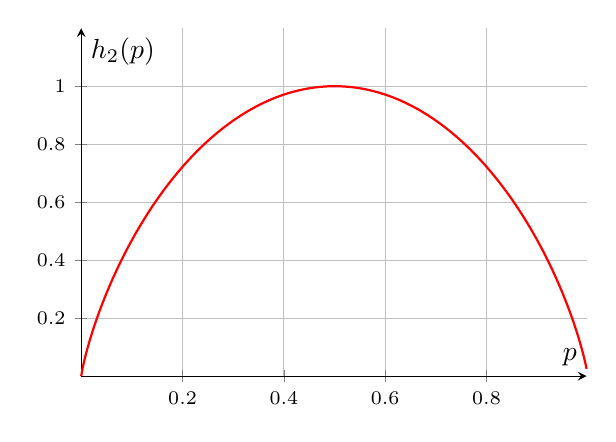
\begin{tikzpicture}
    \begin{axis}[
        xlabel=$p$,
        ylabel=$h_2(p)$,
        domain=0:1,
        samples=400,
        ymin=0,
        ymax=1.2,
        width=8cm,
        height=6cm,
        axis lines=middle,
        grid=major,
        clip=false,
        xtick={0, 0.2, 0.4, 0.6, 0.8, 1},
        ytick={0, 0.2, 0.4, 0.6, 0.8, 1},
        tick label style={font=\scriptsize},
        legend style={at={(0.95,0.95)},anchor=north east, font=\scriptsize},
    ]
    \addplot [red, thick] {-x * log2(x) - (1 - x) * log2(1 - x)};
    \end{axis}
\end{tikzpicture}